\documentclass{article}

\usepackage{graphicx}
\usepackage{tikz}
\usepackage{tikzsymbols}
\usetikzlibrary{calc,patterns,shapes.geometric}
\pagestyle{empty}
\usepackage[margin=0pt]{geometry}
\geometry{papersize={14in,12in}}

\def\centerarc[#1](#2)(#3:#4:#5){\draw[#1] ($(#2)+({#5*cos(#3)},{#5*sin(#3)})$) arc (#3:#4:#5);}

\begin{document}
	\begin{figure}
		\centering
		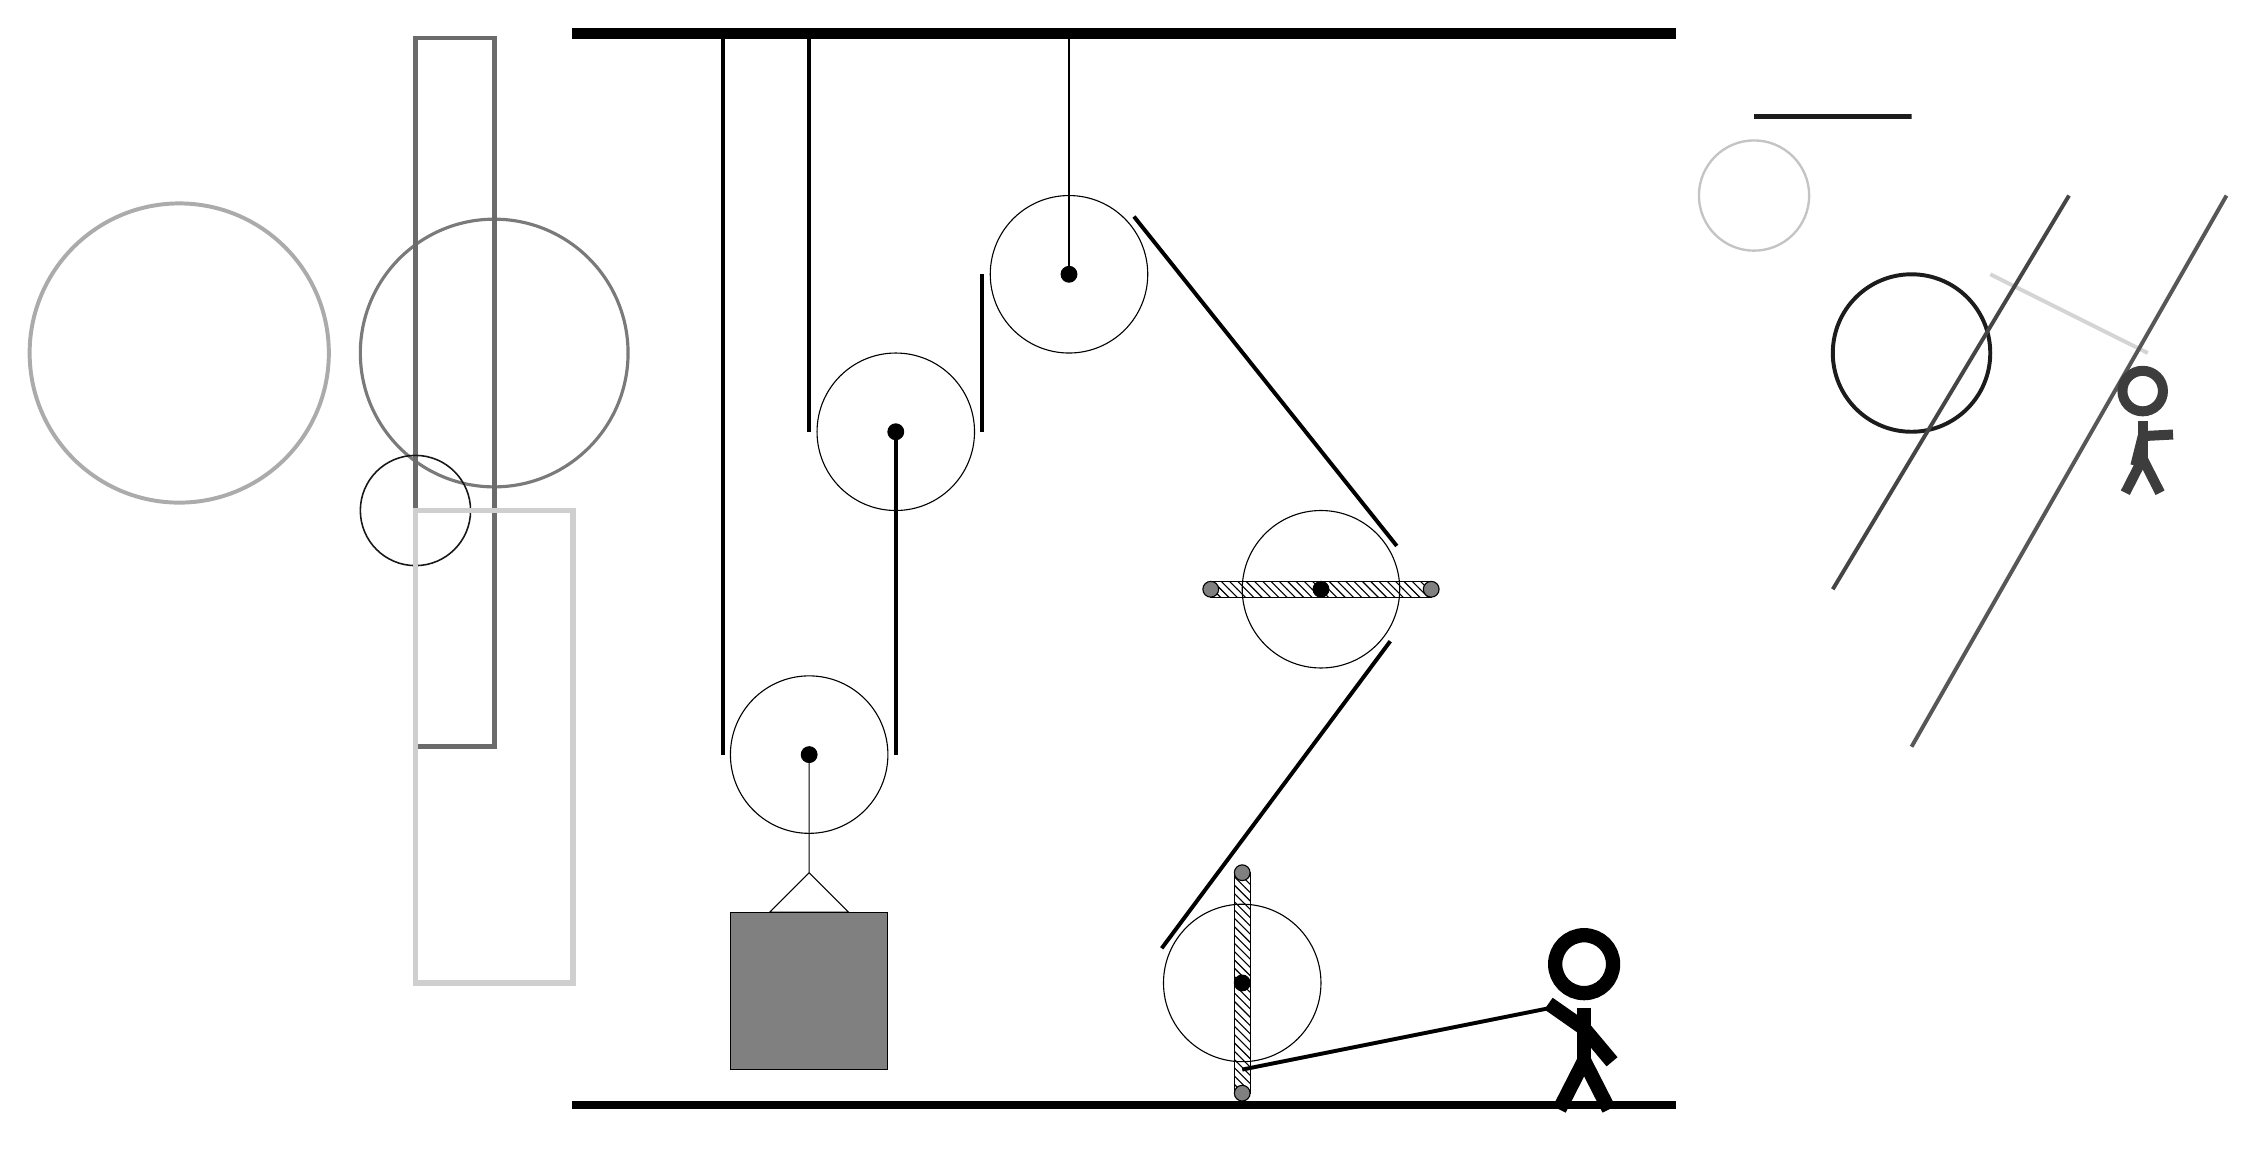
\begin{tikzpicture}
			%%%%% START %%%%%
			
			\draw[fill=black] (-2, 10) rectangle (12, 10.125);
			
			\draw (1, 0.9) circle (1);
			\draw[fill=black] (1, 0.9) circle (0.1);
			
			\draw (2.1, 5.0) circle (1);
			\draw[fill=black] (2.1, 5.0) circle (0.1);
			
			\draw (4.3, 7.0) circle (1);
			\draw[fill=black] (4.3, 7.0) circle (0.1);
			\draw[thick] (4.3, 7.0) -- (4.3, 10);
			
			\draw (6.5, -2) circle (1);
			\draw[fill=black] (6.5, -2) circle (0.1);
			\draw[pattern=north west lines, pattern color=black] (6.4, -0.6) rectangle (6.6, -3.4);
			\draw[fill=black!50] (6.5, -0.6) circle (0.1);
			\draw[fill=black!50] (6.5, -3.4) circle (0.1);
			
			\draw (7.5, 3.0) circle (1);
			\draw[fill=black] (7.5, 3.0) circle (0.1);
			\draw[pattern=north west lines, pattern color=black] (6.1, 3.1) rectangle (8.9, 2.9);
			\draw[fill=black!50] (6.1, 3.0) circle (0.1);
			\draw[fill=black!50] (8.9, 3.0) circle (0.1);
			
			\draw (1, 0.9) -- (1, -0.6) -- (0.5, -1.1) -- (1.5, -1.1) -- (1, -0.6);
			\draw[fill=black!50] (0, -1.1) rectangle (2, -3.1);
			
			\draw[line width=0.5mm] (-0.1, 10) -- (-0.1, 0.9);
			\centerarc[line width=0.5mm](1, 0.9)(180:360:1.1);
			\draw[line width=0.5mm](2.1, 0.9) -- (2.1, 5.0);
			\draw[line width=0.5mm] (1.0, 10) -- (1.0, 5.0);
			\centerarc[line width=0.5mm](2.1, 5.0)(180:360:1.1);
			\draw[line width=0.5mm](3.2, 5.0) -- (3.2, 7.0);
			\centerarc[line width=0.5mm](4.3, 7.0)(35:180:1.1);
			\draw[line width=0.5mm] (5.125, 7.7333) -- (8.4625, 3.55);
			\centerarc[line width=0.5mm](7.5, 3.0)(215:135:-1.1);
			\draw[line width=0.5mm](8.38, 2.34) -- (5.477, -1.56);
			\centerarc[line width=0.5mm](6.5, -2)(-30:100:-1.1);
			\draw[line width=0.5mm](6.5, -3.1) -- (10.5, -2.3);
			
			\node at (10.8, -2.5) {\Strichmaxerl[10][-35][-50]};
			
			\draw[line width=0.5mm, color=black!17](16, 7) -- (18, 6);
			
			\draw [line width=0.4mm, color=black!52](-3, 6) circle (1.7);
			\draw[line width=0.5mm, color=black!66](15, 1) -- (19, 8);
			\draw [line width=0.5mm, color=black!33](-7, 6) circle (1.9);
			\draw[line width=0.6mm, color=black!58] (-4, 10) rectangle (-3, 1);
			\draw[line width=0.6mm, color=black!89] (13, 9) rectangle (15, 9);
			\draw [line width=0.5mm, color=black!89](15, 6) circle (1.0);
			\draw[line width=0.5mm, color=black!73](14, 3) -- (17, 8);
			\node[line width=0.5mm, color=black!76] at (18, 5) {\Strichmaxerl[7][76][3]};
			
			\draw [line width=0.2mm, color=black!91](-4, 4) circle (0.7);
			
			\draw[line width=0.7mm, color=black!19] (-4, 4) rectangle (-2, -2);
			\draw [line width=0.3mm, color=black!23](13, 8) circle (0.7);
			
			\draw[fill=black] (-2, -3.5) rectangle (12, -3.6);
			
			%%%%% END %%%%%
		\end{tikzpicture}
	\end{figure}	
\end{document}